\documentclass{article}
\usepackage[utf8]{inputenc}
\usepackage[margin=0.75in]{geometry}
\usepackage{enumitem}
\usepackage{graphicx}
\usepackage{hyperref}
\usepackage{soul}
\graphicspath{ {./images/} }
\begin{document}
	\begin{center}
    	% MAKE SURE YOU TAKE OUT THE SQUARE BRACKETS
        \topskip 0pt
        \vspace*{\fill}
    		\LARGE{\textbf{System Requirements Analysis}} \\
            \vspace{1em}
            \Large{Engineering Admission Cutoff Learning System} \\
            \vspace{1em}
            \normalsize\textbf{Nikou Kalbali, Maryyam Niazi, Jan Ollers, Yaminah Qureshi} \\
            \normalsize{kalbaln@mcmaster.ca, niazim3@mcmaster.ca, qureshiy@mcmaster.ca, ollersjp@mcmaster.ca} \\
            \vspace{1em}
            \normalsize{Supervisor: Dr. Frantisek Franek} \\
            \vspace{1em}
            \normalsize{Group 2} \\
    \vspace*{\fill}
	\end{center}
	
	\newpage
    \begin{normalsize}
    \tableofcontents
    \newpage
    
    \section{Introduction}

    \subsection{Background}
    A typical university admission process in Ontario takes two steps.
    The first step consists of determining a cutoff threshold to define a subset of all applicants that will be extended an offer if their grade average is not below the cutoff. Some of the offerees become acceptees, while others do not. The second step involves determining the number of applicants the university should be preparing to welcome to their institution and programs. \newline
    \indent In this process, determining an ideal cutoff threshold such that the set of acceptees is of a specific size with some small tolerance is difficult. If the threshold is undervalued, the number of offerees is overshot, typically leading to a set of acceptees that is too large that costs the university financial and space issues from having to deal with too many students.
    If the threshold is overvalued, the number of offerees will be undershot, resulting in a set of acceptees that is too small and costing the university opportunities for revenue and funding from tuition fees and government support. \newline
    \indent This project will use at least two different machine learning approaches trained on previous years of applicant data and their acceptance of offers to an Ontario university to tackle the problem by determining ideal cutoff thresholds based on trends and patterns learned from previous years of data.
    
    \subsection{Purpose}
    	The purpose of this document is to define the requirements of the outlined system which consists of the functionality, intended users, environment, and constraints of the system.
    
    \subsection{Terminology}
    \subsubsection{Offerees}
        The subset of all applicants who will get an offer of acceptance from the university given that their grade average is above the cutoff.
    \subsubsection{Acceptees}
        The subset of offerees who accept the offer received.
    \subsubsection{Grade Percentage Average (GPA)}
        The percentage average of the grades an applicant received as their midterm marks in their last year of high school.
    \subsubsection{Cutoff Threshold}
        The cutoff threshold represented by a grade percentage average that if met by an applicant will result in the applicant receiving an offer of acceptance.
    \subsubsection{University Ranking}
        The ranking of preference given to the university  submitted by an applicant.
	 \subsubsection{Postal Code}
	    The postal code of the location the applicant resides in.
	 \subsubsection{Seat Cap}
	    The maximum number of seats that a university can offer for a program for a particular year.
        
    \section{System Overview}
        \subsection{Use}
        The system will be used for determining cutoff thresholds for two programs at an Ontario university. \newline
        \indent By taking in applicant information from the current admission cycle and using information from previous admission cycles, the cutoff thresholds will be estimated to obtain an ideal number of offerees.
        
        \subsection{Users}
        The primary intended users of the system are the Admissions Committees for Ontario universities. The system may be used as an analysis tool to help them evaluate and/or improve their current admissions process. Further, if we can expand the system and make it applicable to other university program admissions, the admissions committees of these programs will serve as secondary users.

        \subsection {Environment}
        It is intended that the system will be runnable by MAC, Linux/Unix and Windows operating systems as a command-line program. Users will be required to upload the data they would like to input to the system in a directory structure/format as specified and the system will use the data to output a result directly to the terminal/command prompt. Additional files may be created with further information about the result and be stored in a directory structure/format.
   
    \section{Context Diagram}
   \begin{center}
        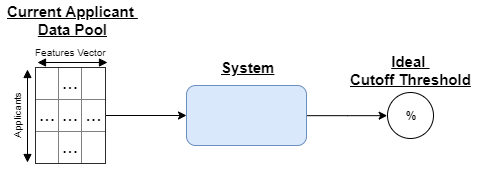
\includegraphics[width=300pt]{images/simpleDiagram}
   \end{center}
   
	\section{Functional Requirements}
	    \subsection{System Data Requirements}
	        The system should be built around 8 years of data which will include applicant pool data (e.g. postal code, university rankings, grade percentage averages, offer status, acceptance status, etc.) and the seat caps for each year.
        \subsection{Input Requirements}
            The system should accept applicant pool data for one year and currently available seating cap for the same year. The applicant pool data includes information about the student postal code, university preference rankings and midterm grade percentage averages.
    	\subsection{Output Requirements}
            The system should output a percentage representing the cutoff threshold that applicants must meet to receive an acceptance offer.
            \begin{itemize}
                \item The system will produce a percentage of up to two decimal places that will not be rounded up.
                \item The number produced must be such that the set of projected acceptees is of a specific size, within a degree of tolerance. This size is influenced by the number of seats that the University wishes to offer for the program for the year. The tolerance is such that the percentage produced to the 0.01 degree should minimize the difference between the number of acceptees and the number of available seats for the program, such that the number of acceptees is not zero \footnote{Universities are not allowed to discriminate based on a grade (i.e. all applicants must be offered an acceptance if they meet the cutoff threshold)}.
            \end{itemize}

    \section{Non-functional Requirements}
    \subsection{Confidentiality}
        The data that will be used to implement and test the system will include sensitive information about students who have applied to two particular programs at a specific university. It is important to make sure this information remains confidential throughout the development of the system. Some measures that will be taken to ensure this include: completely anonymizing the information before use, restricting the system from outputting or storing any data that could compromise student confidentiality, and restricting users of the program from accessing data they have not provided themselves. \footnote{Questions regarding confidentiality of the data may be directed to \href{cas.mcmaster.ca/~franek/}{Dr. Frantisek Franek}}
        
    \subsection{Reliability}
        The system should produce an accurate and realistic result for all data that meets the required input data structure.

    \subsection{Data Integrity}
        The data taken in as input to the system should not be modified before it is used by the system.

    \subsection{Reusability}
        Ability to use the system over multiple years of data, as long as admission processes and policies do not significantly change.
  
    \section{System Constraints}
        \begin{itemize}
            \item The scope of the system is limited to two particular programs at a specific university as the data that has been provided on which the system will be trained is for these particular programs. For this reason, the system is limited to producing results for that university's admissions. However, in the future, expanding this project to more universities and programs is a possibility.
            \item Although using more data to develop the system may result in increased accuracy, only data from the previous 8 years of applicants are available as universities are required to maintain applicant confidentiality. For this reason, the system is constrained to learning from 8 years of previous applicant information.
        \end{itemize}

\end{normalsize}
\end{document}
